\documentclass[11pt]{article}
\usepackage[T1]{fontenc}
\usepackage{lmodern}
\usepackage[margin=1in]{geometry}
\usepackage{amsmath,amssymb,amsthm,mathtools}
\usepackage{microtype,booktabs,flafter}
\usepackage{tikz}
\usetikzlibrary{arrows.meta,positioning,calc,decorations.pathreplacing}
\usepackage[hidelinks]{hyperref}
\hypersetup{pdftitle={Polynomial-Time Unitary Synthesis from a Boolean Oracle},pdfauthor={OpenAI}}
\newcommand{\C}{\mathbb C}
\newcommand{\R}{\mathbb R}
\newcommand{\N}{\mathbb N}
\newcommand{\Z}{\mathbb Z}
\newcommand{\E}{\mathbb E}
\newcommand{\ket}[1]{\lvert #1\rangle}
\newcommand{\bra}[1]{\langle #1\rvert}
\newcommand{\ip}[2]{\langle #1,#2\rangle}
\newcommand{\norm}[1]{\lVert #1\rVert}
\newcommand{\id}{\mathrm{id}}
\DeclareMathOperator{\Tr}{Tr}
\DeclareMathOperator{\diag}{diag}
\DeclareMathOperator{\supp}{supp}
\DeclareMathOperator{\poly}{poly}
\newtheorem{theorem}{Theorem}[section]
\newtheorem{lemma}[theorem]{Lemma}
\newtheorem{proposition}[theorem]{Proposition}
\newtheorem{corollary}[theorem]{Corollary}
\theoremstyle{definition}
\newtheorem{definition}[theorem]{Definition}
\theoremstyle{remark}
\newtheorem{remark}[theorem]{Remark}
\numberwithin{equation}{section}
\title{Polynomial-Time Unitary Synthesis\\ from a Boolean Oracle}
\author{OpenAI}
\date{October 5, 2026}
\begin{document}
\maketitle
\begin{abstract}
We give a positive answer to the constant-error formulation of the
Aaronson--Kuperberg unitary synthesis problem. For every $n$, a quantum oracle
circuit generated in polynomial time from $n$ alone can approximate the channel
of every $n$-qubit unitary to full diamond-norm error at most $1/2$, after a
suitable Boolean oracle is chosen. Using the fixed gates
$H,T,T^\dagger,\mathrm{CNOT}$, the circuit has polynomially many qubits,
elementary gates, and oracle calls, and its oracle queries have polynomial
length. The oracle may depend on the target unitary; the theorem does not give
an efficient classical procedure for constructing it.
\end{abstract}
\section{Introduction}\label{sec:introduction}
A classical description of a quantum operation can be much longer than the
register on which the operation acts.  Oracle access offers a way to separate
the size of that description from the work needed to use it.  The unitary
synthesis problem asks whether every operation on $n$ qubits can be performed
in quantum polynomial time when a suitable classical description is available
through coherent queries to a Boolean function.  Aaronson and Kuperberg posed
this question in 2007~\cite[Section~7, Problem~(4)]{AK2007}; Aaronson later
highlighted it among open problems in quantum query
complexity~\cite[Problem~6]{Aaronson2021}.

We give a positive answer to the constant-error formulation.  One circuit,
determined only by $n$, works for every $n$-qubit unitary after an appropriate
Boolean oracle is chosen.  The circuit uses polynomially many gates, qubits,
and queries, and each query has polynomial length.  The error bound holds for
arbitrary input states, including states entangled with a reference system.

\subsection{Model and main result}
We use the fixed elementary gate set
\[
 H=\frac1{\sqrt2}\begin{pmatrix}1&1\\1&-1\end{pmatrix},
 \qquad T=\begin{pmatrix}1&0\\0&e^{i\pi/4}\end{pmatrix},
 \qquad T^\dagger,\qquad \mathrm{CNOT},
\]
where $\mathrm{CNOT}\ket{a,b}=\ket{a,a\oplus b}$.  A Boolean oracle
$f:\{0,1\}^m\to\{0,1\}$ supplies the gate
\begin{equation}\label{intro:oracle}
 O_f\ket{x,b}=\ket{x,b\oplus f(x)}.
\end{equation}
A circuit receives an $n$-qubit input and workspace initialized to zero.  Its
output channel is obtained by retaining $n$ designated qubits and tracing out
the remaining qubits.

For a unitary $U$, write $\mathcal U(\rho)=U\rho U^\dagger$.  Our convention for
channel error is the full diamond norm: if $\Phi$ is another channel on $n$
qubits, then
\begin{equation}\label{intro:diamond}
 \norm{\Phi-\mathcal U}_\diamond
 =\sup_{\rho}\norm{\bigl((\Phi-\mathcal U)\otimes\id_R\bigr)(\rho)}_1,
 \qquad \norm{X}_1=\Tr\sqrt{X^\dagger X},
\end{equation}
where $R$ is an $n$-qubit reference register and $\rho$ ranges over density
operators on the input and $R$.  Thus the norm in
\eqref{intro:diamond} has no factor of $1/2$.

\begin{theorem}[Polynomial-time unitary synthesis]\label{thm:main}
There are a polynomial $p$ and a deterministic classical algorithm which, on
input $1^n$ for any integer $n\ge1$, outputs in time at most $p(n)$ a quantum
oracle circuit $A_n$ with the following properties.  The circuit uses the gates
$H,T,T^\dagger,\mathrm{CNOT}$ and a single Boolean oracle of input length
$m(n)\le p(n)$.  Its total number of qubits, elementary gates, and oracle calls
are each at most $p(n)$.  For every unitary $U\in U(2^n)$ there is a function
$f:\{0,1\}^{m(n)}\to\{0,1\}$ for which the output channel $\Phi_{n,f}$ of
$A_n^{O_f}$ satisfies
\[
 \norm{\Phi_{n,f}-\mathcal U}_\diamond\le\frac12.
\]
\end{theorem}

The quantifiers are essential.  The circuit and its resource bounds depend
only on $n$; the oracle may depend on $U$.  There is no restriction on the
truth-table size or classical circuit complexity of $f$, and no prescribed
encoding of $U$ that the algorithm must use.  The theorem is an existence
statement about such an encoding.  It does not give an efficient classical
procedure for constructing the oracle from a description of $U$.

\subsection{Earlier work}
State synthesis provides a useful comparison.  It asks for preparation of one
specified state from a fixed input, whereas unitary synthesis must act
coherently on every input.  Irani, Natarajan, Nirkhe, Rao, and Yuen obtained
one- and two-query state-synthesis results with polynomial
space~\cite{INNRY2022}.  Rosenthal subsequently gave uniform polynomial-size
state-synthesis circuits using one Boolean query when workspace may be
discarded, and four queries when it must be returned to
zero~\cite{Rosenthal2024}.  These results do not immediately implement an
arbitrary unitary: preparing a chosen column while retaining its input label
does not erase that label coherently on a superposition of inputs.

For unitary synthesis, Rosenthal gave a running-time upper bound of order
$2^{n/2}$ up to polynomial factors, using an oracle suited to the target
unitary~\cite{Rosenthal2026}.  In the other direction, Lombardi, Ma, and Wright
proved a general one-query lower bound, which also rules out polynomially
many parallel queries of polynomial length~\cite{LMW2024}.  Dong, Lombardi,
and Ma obtained explicit one-query separations for several structured
families of unitaries~\cite{DLM2026}.  These lower bounds leave open the use of
multiple queries interleaved with quantum computation, as in the construction
here.

Nehoran and Yuen recently showed that every unitary in dimension $N$ admits a
constant-query implementation using three diagonal-phase queries, or six
Boolean queries~\cite{NY2026}.  The diagonal-phase version uses
$O(N\log\log(N/\varepsilon))$ query qubits for operator-norm error
$\varepsilon$.  For $N=2^n$, this is exponential
in the number of input qubits.  Theorem~\ref{thm:main} concerns polynomial
total resources, including the width of the oracle interface.  The distinction
between query count and query width is therefore indispensable when comparing
these results.

\subsection{The reduction}
The central construction replaces synthesis of a $d$-dimensional unitary by
synthesis of one smaller, coherently controlled unitary.  Each reduction
removes a fraction at least $1/\poly(n)$ of the dimension, so only polynomially
many reductions are needed even when $d=2^n$.  The smaller synthesis circuit is
used exactly once at each step.  This last property prevents the recursion
from producing an exponentially large circuit.

Here is the mechanism.  After changes of basis built from permutations, diagonal signs, and Walsh
transforms, write the current unitary as
\[
 V=\begin{pmatrix}A&B\\C&D\end{pmatrix},\qquad \norm{D}\le\frac34,
\]
where $D$ has the dimension to be removed.  Random diagonal signs and Walsh
transforms supply this contracting block.  The needed norm estimate is proved
by a Gaussian moment argument in Section~\ref{sec:contraction}.
For a diagonal unitary $Z$ on the removed coordinates, close the lower output
back into the lower input through $Z$.  Solving the resulting linear equation
gives
\[
 F=A+BZ(I-DZ)^{-1}C.
\]
Conservation of norm makes $F$ unitary on the remaining coordinates.  This is
the familiar transfer-function construction for a unitary block
matrix~\cite{FKK2009}; our task is to turn it into a circuit reduction.

For that purpose we construct two maps, $\mathcal E$ and $\mathcal R$, from
the original space into a register holding $Z$ together with a smaller state.
They satisfy an approximate intertwining relation
\[
 \widetilde F\mathcal E\approx\mathcal R V,
\]
where $\widetilde F$ applies the corresponding $F$ controlled by the $Z$
register.  Both maps are nearly isometric.  They come from truncating the
forward and backward geometric series associated with $(I-DZ)^{-1}$.
Averaging over a common phase cancels unequal degrees, and unitarity makes
the remaining Gram-matrix sums telescope.  The errors decay exponentially
with the truncation length.

The implementability of these maps depends on their Fourier coefficients.
We assign to each removed coordinate $i$ the frequency vector
$(1,i,\ldots,i^L)$, where $L$ is the truncation length.  The Fourier frequency of a product of at most
$L$ phases records a multiset of coordinates through its power sums.  For
an input on a removed coordinate, each nonzero coefficient records a
multiset containing that coordinate.  Inputs on the remaining coordinates
contribute only at frequency zero, with one input column per output coordinate.  Consequently every row of either
coefficient matrix has at most $L$ nonzero entries, although a column may
be dense.  This row bound lets a
circuit coherently erase the input index after preparing a column.  Amplitude
amplification then converts the resulting scaled map into an approximation
to the required encoding.  The two encoders surround a single call to the
smaller unitary, as shown in Figure~\ref{fig:recursion}.

The feedback identity, the matching forward and backward encodings, and the
multiset argument are developed in Section~\ref{sec:fields}.
Section~\ref{sec:encoders} proves the circuit implementation for a general
nearly isometric matrix with few nonzero entries per row, and
Section~\ref{sec:recursion} assembles the recursion and bounds its resources.
These intermediate constructions are stated separately so that their
hypotheses and uses remain visible.

We first work with controlled single-qubit gates whose entries may be
arbitrary functions of their control bits.  Section~\ref{sec:slots} defines
these programmable gates and the elementary operations they provide.
Section~\ref{sec:compilation} replaces every such gate by a polynomial-length
word over the fixed gate set, read from one Boolean oracle.  This compilation
preserves relative phases between different control values.  Throughout the
proof, errors are measured on the subspace where the input workspace is zero;
a final isometry estimate yields the diamond-norm guarantee in
Theorem~\ref{thm:main}.

\section{Controlled tasks and programmable slots}\label{sec:slots}

We first construct circuits whose one-qubit gates can be selected from arbitrary
tables. This separates the geometry of the circuit from the information about
the target unitary. Section~\ref{sec:compilation} will store finite approximations
to these tables in one Boolean oracle.

All vector norms are Euclidean, and $\norm{A}$ denotes the operator norm of a
linear map $A$. Both $A^*$ and $A^\dagger$ denote its adjoint. We never minimize
this norm over scalar phases. For
$1\le d\le 2^n$, write
\[
 \mathcal H_d=\operatorname{span}\{\ket{0},\ldots,\ket{d-1}\}
 \subseteq (\C^2)^{\otimes n}.
\]
The recursion must synthesize many unitaries coherently. Its input therefore
includes a \emph{label register} with basis $\ket{\lambda}$,
$\lambda\in\{0,1\}^t$, and its prescribed action is
\[
 \mathcal U=\sum_{\lambda}\ket{\lambda}\bra{\lambda}\otimes U_\lambda,
 \qquad U_\lambda\colon\mathcal H_d\longrightarrow\mathcal H_d
 \text{ unitary}.
\]
Let $\iota$ append all working qubits in state $\ket{0}$. A circuit $C$
solves this controlled task with error $\delta$ if
\begin{equation}\label{slot:clean-error}
 \norm{C\iota-\iota\mathcal U}\le\delta.
\end{equation}
Thus the estimate includes restoration of the working qubits, and is uniform
over superpositions of labels. No behavior is prescribed outside the input
subspace $\operatorname{span}\{\ket{\lambda}\}\otimes\mathcal H_d$.
The same estimate holds after tensoring with the identity on any further
register, because operator norm is unchanged by that operation.

A \emph{programmable slot} specifies one target qubit and an ordered list of
other qubits as controls. Given a table of matrices $W_y\in U(2)$, its action is
\begin{equation}\label{slot:definition}
 \sum_{y\in\{0,1\}^c}\ket{y}\bra{y}\otimes W_y,
\end{equation}
where $c$ is the number of controls. A \emph{circuit skeleton} specifies the
registers, targets, and control lists of its slots, but leaves their tables
unspecified. The tables may depend on the target unitaries. Their contents
are not part of the skeleton that the uniform generator must produce.
Reversing a skeleton reverses its slot order and replaces every table by its
adjoint table.
Slots are uniformly controlled one-qubit gates, or quantum multiplexors,
in the terminology of~\cite{BVMS2005}.

Every diagonal unitary on $u\ge1$ qubits uses a single slot: choose one of
the qubits as target and put the two diagonal entries for each value of the
other $u-1$ bits in the corresponding $2\times2$ diagonal table entry.
Additional labels can be included among the controls. In particular,
reflections in subspaces spanned by specified computational basis states
take one slot. A phase depending only on labels can be applied to a zero
working qubit, or by scalar matrices on an existing target qubit.

\begin{lemma}[State preparation]\label{slot:preparation}
For every $u\ge1$ there is a skeleton of $u+1$ slots that maps
$\ket{\lambda}\ket{0^u}$ to $\ket{\lambda}\ket{a_\lambda}$ for any prescribed
family of unit vectors $a_\lambda\in\C^{2^u}$. Its structure depends only on
the register sizes.
\end{lemma}

\begin{proof}
Fix a label and write $a=\sum_x a_x\ket{x}$. For a binary prefix $p$, let
$P(p)=\sum_{x\text{ extending }p}|a_x|^2$. Process the bits from first to last.
At the next bit, controlled on the preceding prefix $p$, apply a real
rotation whose first column is
\[
 \begin{pmatrix}
  \sqrt{P(p0)/P(p)}\\[2pt]
  \sqrt{P(p1)/P(p)}
 \end{pmatrix}
 \quad\text{when }P(p)>0.
\]
Choose any rotation when $P(p)=0$. After $u$ such slots the amplitude at $x$
is $|a_x|$. One diagonal slot then supplies the phases of the $a_x$, choosing
arbitrary phases at zero entries. Including $\lambda$ among the controls
makes all these choices simultaneously. This is the usual conditional
rotation construction for state preparation; here an entire uniformly
controlled rotation is counted as one slot; see~\cite{MVBS2005,BVMS2005}.
\end{proof}

\begin{lemma}[Basis permutations]\label{slot:permutation}
Any family of permutations of the $2^u$ computational basis states can be
implemented with $5u$ slots and $u$ temporary qubits that start and finish
at zero. The skeleton is independent of the permutations.
\end{lemma}

\begin{proof}
For the permutation $\pi_\lambda$, use $u$ slots to write its image bitwise
into a temporary register:
\[
 \ket{\lambda}\ket{x}\ket{0}
 \longmapsto \ket{\lambda}\ket{x}\ket{\pi_\lambda(x)}.
\]
Each slot chooses either $I$ or the bit flip, controlled on $\lambda$ and
$x$. Next use $u$ slots to xor $\pi_\lambda^{-1}(y)$ into the first register,
controlled on the second register $y$. The two registers become
$\ket{0}\ket{\pi_\lambda(x)}$. Swap them using three CNOTs per pair of bits.
\end{proof}

The same convention makes a Fourier transform inexpensive. We use the
positive-phase transform, so that a frequency basis vector becomes its
character in the computational basis.

\begin{lemma}[Fourier transforms]\label{slot:fourier}
The unitary
\[
 \ket{x}\longmapsto 2^{-b/2}\sum_{z=0}^{2^b-1}
       e^{2\pi i xz/2^b}\ket{z}
\]
on $b\ge1$ qubits has a uniformly generated skeleton with $O(b)$ slots.
Products of such transforms have a number of slots linear in their total
register width.
\end{lemma}

\begin{proof}
Write the input integer as $x$. Process its bits in decreasing order of
place value. At the bit of place value $2^{b-1-j}$, apply $H$, then a
diagonal slot controlled on the still unprocessed lower bits. Give the
state $1$ the additional phase that, together with its sign from $H$,
makes the ratio of its two amplitudes equal to
$e^{2\pi i x/2^{b-j}}$. Bits above the current bit contribute integral
multiples of $2\pi$ to this expression, and are no longer needed as
controls. The resulting bit is the Fourier output bit of place value
$2^j$. A final reversal of bit order gives the stated transform. There are
two slots per processed bit and $O(b)$ CNOTs for the reversal.
\end{proof}

These constructions retain the scalar phase of every label branch. This is
essential: phases that would be irrelevant for one isolated unitary become
relative phases when the same operation is controlled by a quantum register.

\section{Producing a contracting block}\label{sec:contraction}

The reduction will remove a small group of indices from the synthesis problem.
For its geometric series to converge rapidly, the corresponding diagonal block
of the unitary must have norm bounded away from one.  We now obtain such a block
using only permutations, diagonal signs, and Walsh--Hadamard transforms.  All
these transformations have short programmable-slot implementations.

We first record the matrix estimate needed to choose the signs.  A
\emph{Rademacher variable} takes the values $1$ and $-1$ with equal probability.
The following elementary moment argument is a finite-dimensional form of the
noncommutative Khintchine estimate; see Tropp~\cite[Sections~6--7]{Tropp2018}
for the Gaussian integration-by-parts and trace-product method.  We include
the proof with the constants used below.

\begin{lemma}[A matrix sign estimate]\label{contract:moment}
Let $L_1,\ldots,L_q$ be Hermitian $h\times h$ matrices, and let
$\varepsilon_1,\ldots,\varepsilon_q$ be independent Rademacher variables.
Set $v=\norm{\sum_i L_i^2}$.  For every integer $a\geq1$,
\begin{equation}\label{contract:sign-bound}
 \E\norm{\sum_{i=1}^q\varepsilon_iL_i}
 \leq 2h^{1/(2a)}\sqrt{(2a-1)v}.
\end{equation}
\end{lemma}

\begin{proof}
We first replace the signs by independent standard real Gaussians $g_i$ and
write $X=\sum_i g_iL_i$.  Gaussian integration by parts, applied to this matrix
polynomial, gives
\begin{equation}\label{contract:ibp}
 \E\Tr X^{2a}
 =\sum_{i=1}^q\sum_{l=0}^{2a-2}
   \E\Tr\bigl(L_iX^lL_iX^{2a-2-l}\bigr).
\end{equation}
Indeed, write the first factor of $X^{2a}$ as $\sum_i g_iL_i$, use
$\E[g_iP(g)]=\E[\partial_iP(g)]$, and differentiate each of the remaining
$2a-1$ factors in turn.

Put $m=2a-2$.  For a fixed Hermitian $X$, diagonalize it with real eigenvalues
$\lambda_j$.  In this basis, for $m>0$,
\begin{align*}
 \Tr(L_iX^lL_iX^{m-l})
 &=\sum_{j,k}|(L_i)_{jk}|^2\lambda_k^l\lambda_j^{m-l}\\
 &\leq\sum_{j,k}|(L_i)_{jk}|^2
   \left(\frac lm|\lambda_k|^m+
              \frac{m-l}{m}|\lambda_j|^m\right)
 =\Tr(L_i^2X^m).
\end{align*}
The inequality is the weighted arithmetic--geometric mean inequality after
taking absolute values.  The last equality uses the symmetry
$|(L_i)_{jk}|^2=|(L_i)_{kj}|^2$ and the evenness of $m$.
For $m=0$ the same assertion is equality.  Since $X^m$ is positive semidefinite
and $\sum_iL_i^2\preceq vI$, equation~\eqref{contract:ibp} implies
\[
 \E\Tr X^{2a}\leq(2a-1)v\,\E\Tr X^{2a-2}.
\]
Iterating from $\Tr I=h$ yields
\[
 \E\Tr X^{2a}
 \leq h(2a-1)!!\,v^a
 \leq h(2a-1)^a v^a.
\]
Here $(2a-1)!!=1\cdot3\cdots(2a-1)$.  Therefore
\begin{equation}\label{contract:gaussian-bound}
 \E\norm X
 \leq\bigl(\E\norm X^{2a}\bigr)^{1/(2a)}
 \leq h^{1/(2a)}\sqrt{(2a-1)v}.
\end{equation}

To return to signs, write $g_i=\varepsilon_i t_i$, where the $t_i=|g_i|$ are
independent of the signs and have common mean $\mu=\sqrt{2/\pi}$.  Conditional
Jensen gives
\[
 \mu\,\norm{\sum_i\varepsilon_iL_i}
 \leq\E_t\norm{\sum_i\varepsilon_i t_iL_i}.
\]
Average over the signs, apply~\eqref{contract:gaussian-bound}, and use
$\mu^{-1}<2$.
\end{proof}

Fix throughout the construction
\begin{equation}\label{contract:parameters}
 M=4096(n+1)^2,\qquad r=\frac34.
\end{equation}
For an integer $2\leq d\leq2^n$, let $q$ be the largest power of two not
exceeding $d$, and define
\begin{equation}\label{contract:orders}
 s=\max\{1,\lfloor q/M\rfloor\},\qquad k=d-s.
\end{equation}
We call the first $k$ indices \emph{ports} and the last $s$ indices
\emph{internal indices}.  Both groups are nonempty.

\begin{proposition}[A block of uniformly small norm]\label{contract:block}
For every unitary $U$ on $\C^d$, there are unitaries $P_{\mathrm L}$ and
$P_{\mathrm R}$ on $\C^d$ such that
\begin{equation}\label{contract:block-form}
 V=P_{\mathrm L}UP_{\mathrm R}
 =\begin{pmatrix}A&B\\C&D\end{pmatrix},
 \qquad \norm D\leq r,
\end{equation}
where the block sizes are $k,s$ from~\eqref{contract:orders}.
The transformations $P_{\mathrm L},P_{\mathrm R}$ and their inverses have
implementations using $O(n)$ programmable slots and $O(n)$ clean working
qubits, with a structure determined by $n,d$.  The same structure works
simultaneously for any family $U_\lambda$, using the label $\lambda$ as an
additional control.
\end{proposition}

\begin{proof}
If $s=1$, the last column of $U$ has an entry of modulus at most $1/\sqrt d$.
A row permutation moves this entry to the last position.  The resulting
one-dimensional block satisfies $\norm D\leq1/\sqrt d<3/4$, and the permutation
has the claimed slot implementation by Lemma~\ref{slot:permutation}.

Suppose $s>1$.  Let $M_0$ be the last-by-last $q\times q$ submatrix of $U$;
it is a contraction.  Set
$H_q=H^{\otimes\log_2q}$, and let $W$ consist of its last $s$ columns.  We
will choose diagonal sign matrices $E_1,E_2$ on $\C^q$ and use
$H_qE_1$ on the left and $E_2H_q$ on the right, acting as the identity on the
remaining $d-q$ indices.  The resulting internal block is
\begin{equation}\label{contract:D-signs}
 D=W^*E_1C',\qquad C'=M_0E_2W.
\end{equation}
We choose $E_2$ first to bound the entries of $C'$, then choose $E_1$ to
bound the operator norm of $D$.

For independent signs in $E_2$, each entry of $C'$ is a sign sum
$\sum_j\varepsilon_j\alpha_j$ with $\sum_j|\alpha_j|^2\leq1/q$.
For completeness, a real sign sum with squared coefficient sum at most $1/q$
satisfies
\[
 \E\exp\left(t\sum_j\varepsilon_j a_j\right)
 =\prod_j\cosh(ta_j)\leq\exp(t^2/(2q)).
\]
Markov's inequality, optimized over $t$, bounds its two-sided tail at $u$ by
$2e^{-qu^2/2}$.  Applying this to the real and imaginary parts shows
\[
 \Pr\left(\left|\sum_j\varepsilon_j\alpha_j\right|\geq u\right)
 \leq4e^{-qu^2/4}.
\]
There are $qs$ entries.  With $u=4\sqrt{(n+1)/q}$, the union-bound failure
probability is at most
\[
 4qs e^{-4(n+1)}\leq4\cdot2^{2n}e^{-4(n+1)}<1.
\]
We may therefore fix $E_2$ such that every entry of $C'$ has modulus at most
$4\sqrt{(n+1)/q}$.  Also $\norm{C'}\leq1$.

Let $h_i,c_i$ be row $i$ of $W,C'$, respectively, regarded as row vectors.
Then
\[
 \norm{h_i}^2=s/q,\qquad
 \norm{c_i}^2\leq v:=16s(n+1)/q.
\]
Choosing independent signs $\varepsilon_i$ for $E_1$, write
\[
 D=\sum_i\varepsilon_i h_i^*c_i,
 \qquad
 L_i=\begin{pmatrix}0&h_i^*c_i\\c_i^*h_i&0\end{pmatrix}.
\]
The two diagonal blocks of $\sum_iL_i^2$ satisfy
\[
 \sum_i\norm{c_i}^2h_i^*h_i\preceq vW^*W=vI_s,
 \qquad
 \sum_i\norm{h_i}^2c_i^*c_i
 =\frac sq C'^*C'\preceq\frac sq I_s\preceq vI_s.
\]
The norm of $\sum_i\varepsilon_iL_i$ equals $\norm D$.  Apply
Lemma~\ref{contract:moment} with $h=2s$ and $a=n+1$.  Since
$(2s)^{1/(2n+2)}\leq\sqrt2$, we obtain
\[
 \E\norm D
 \leq 2\sqrt2\sqrt{2(n+1)\,16s(n+1)/q}
 =16(n+1)\sqrt{s/q}
 \leq\frac14.
\]
The last inequality uses $s\leq q/M$.  Some choice of $E_1$ consequently
satisfies $\norm D\leq1/4$, which is more than required.

It remains to check the circuit structure.  A permutation on the $n$-bit
index register moves the last $q$ valid indices to the first $q$ valid
indices, an aligned $q$-element block.  On that block, $H_q$ uses at most
$n$ Hadamard slots, controlled on
the remaining bits; each diagonal sign matrix uses one diagonal slot.  Undo
the permutation afterward.  Lemma~\ref{slot:permutation} supplies clean
$O(n)$-slot implementations of the permutations.  All operations preserve
the valid $d$-dimensional subspace and are extended unitarily to unused index
states.  Labels change only the row permutation or diagonal-sign tables,
so the same slot structure works for every $U_\lambda$.
\end{proof}

The random signs are used only to prove that suitable tables exist.
Each label may use its own choices; the resulting slot circuit is deterministic.
The size of the removed block is large enough to make recursion short.
\begin{lemma}[Dimension decrease]\label{contract:depth}
For the parameters in~\eqref{contract:orders}, $s\geq d/(4M)$.
Starting at any $d\leq2^n$ and repeatedly replacing $d\geq2$ by $d-s$, one
reaches $d=1$ in fewer than
\begin{equation}\label{contract:J}
 J=8M(n+1)
\end{equation}
steps.
\end{lemma}

\begin{proof}
If $q/M\geq2$, then
$s=\lfloor q/M\rfloor\geq q/(2M)>d/(4M)$, because $d<2q$.
If $q/M<2$, then $s=1$ and $d<2q<4M$, with the same conclusion.
Thus every nontrivial step multiplies the order by at most $1-1/(4M)$.
If there were $J$ such steps, their final order would be at most
\[
 2^n(1-1/(4M))^J
 \leq2^n e^{-J/(4M)}
 =2^n e^{-2(n+1)}<1,
\]
contrary to its being a positive integer.
\end{proof}

\section{Fourier fields for a smaller unitary}\label{sec:fields}

Let $d=k+s\le 2^n$, with $k,s\ge1$, and suppose that
\begin{equation}\label{fields:block}
 V=\begin{pmatrix}A&B\\ C&D\end{pmatrix}\in U(d),
 \qquad \norm{D}\le r<1,\quad r\ge0.
\end{equation}
The first $k$ coordinates are the ports and the last $s$ coordinates are
internal. We will associate to $V$ a family of $k$-dimensional unitaries
$F(z)$ and two nearly isometric maps from $\C^d$ into the space of
port-valued functions of $z$. These maps intertwine $V$ with the controlled
application of $F(z)$. Their Fourier coefficients will have few nonzero
entries in each row, which makes the maps implementable by slots.

\subsection{Closing the internal coordinates}

For the moment let $Z$ be any diagonal unitary of order $s$. Given a port
input $u\in\C^k$, feed the internal output $v\in\C^s$ back into the
internal input through $Z$. If $y\in\C^k$ is the port output, the equation
$V(u,Zv)=(y,v)$ becomes
\[
 y=Au+BZv,\qquad v=Cu+DZv.
\]
Since $\norm{DZ}<1$, the second equation has the unique solution $v=Xu$,
and the first then gives $y=Fu$, where
\begin{equation}\label{fields:feedback}
 X=(I-DZ)^{-1}C,\qquad F=A+BZX,
 \qquad
 E=\begin{pmatrix}I_k\\ ZX\end{pmatrix},\qquad
 O=\begin{pmatrix}F\\ X\end{pmatrix}.
\end{equation}
Thus $Eu$ and $Ou$ collect the full input and output of $V$ after the
internal coordinates have been closed.
For a scalar phase $Z=zI$, this is the standard transfer function of a
unitary block matrix; see \cite[Section~3]{FKK2009}. The same conservation
of norm proves unitarity with independently chosen diagonal phases.

\begin{lemma}\label{fields:unitary}
For the unitary block matrix in \eqref{fields:block} and any diagonal
unitary $Z$, the matrix $F$ in \eqref{fields:feedback} is unitary.
If
\begin{equation}\label{fields:R}
 R=OF^*=\begin{pmatrix}I_k\\ Y\end{pmatrix},
 \qquad Y=XF^*,
\end{equation}
then
\begin{equation}\label{fields:exact}
 FE^*=R^*V,
 \qquad
 Y=(I-Z^*D^*)^{-1}Z^*B^*.
\end{equation}
\end{lemma}

\begin{proof}
The definitions give $VE=O$. Consequently,
\[
 I_k+X^*X=E^*E=O^*O=F^*F+X^*X,
\]
so $F^*F=I_k$. Because $F$ is square, it is unitary. Thus $OF^*$ has
the stated top block, and $V^*R=EF^*$. Taking adjoints proves the first
identity in \eqref{fields:exact}. Comparing the bottom blocks of
$V^*R=EF^*$ gives
\[
 B^*+D^*Y=ZY.
\]
Multiplication by $Z^*$ and $\norm{Z^*D^*}\le r<1$ give the second identity.
\end{proof}

\subsection{Truncation and averaging}

Fix an integer truncation length $L\ge1$, and set
\begin{equation}\label{fields:parameters}
 b=nL+\lceil\log_2(L+1)\rceil,\qquad
 \mathcal G=(\Z/(2^b))^{L+1}.
\end{equation}
For $w,z\in\mathcal G$, write
\[
 \chi_w(z)=\exp(2\pi i\,w\cdot z/2^b).
\]
Number the internal coordinates by $i=1,\ldots,s$ and put
\begin{equation}\label{fields:phases}
 v_i=(1,i,i^2,\ldots,i^L)\in\mathcal G,
 \qquad Z(z)=\diag\bigl(\chi_{v_1}(z),\ldots,\chi_{v_s}(z)\bigr).
\end{equation}
The constant first coordinate of $v_i$ gives all diagonal entries of $Z(z)$
a common phase when the first coordinate of $z$ varies. Averaging that phase
will separate terms of different lengths in the truncated series. The
remaining coordinates record power sums: the Fourier frequency of a product
of at most $L$ phases will determine its multiset of internal indices, as proved in
Proposition~\ref{fields:sparsity}. These two properties will give the norm
bound and the row bound, respectively.

Apply Lemma~\ref{fields:unitary} at each $z$ to obtain $F(z),E(z),R(z)$.
Truncate the two Neumann expansions by defining
\begin{equation}\label{fields:truncations}
 E_L(z)=\begin{pmatrix}
 I_k\\[2pt] \displaystyle\sum_{\ell=0}^{L-1}Z(DZ)^\ell C
 \end{pmatrix},\qquad
 R_L(z)=\begin{pmatrix}
 I_k\\[2pt] \displaystyle\sum_{\ell=0}^{L-1}(Z^*D^*)^\ell Z^*B^*
 \end{pmatrix}.
\end{equation}
Here and below, products containing $Z$ are evaluated at the same $z$.
Since every block of a unitary has norm at most one,
\begin{equation}\label{fields:tails}
 \norm{E_L(z)-E(z)},\ \norm{R_L(z)-R(z)}
 \le \tau,\qquad \tau=\frac{r^L}{1-r}.
\end{equation}

Define the field maps $\mathcal E_L,\mathcal R_L:
\C^d\longrightarrow\C^{\mathcal G}\otimes\C^k$ by
\begin{equation}\label{fields:maps}
 \mathcal E_L x=\frac1{\sqrt{|\mathcal G|}}
   \sum_{z\in\mathcal G}\ket z\otimes E_L(z)^*x,
 \qquad
 \mathcal R_L x=\frac1{\sqrt{|\mathcal G|}}
   \sum_{z\in\mathcal G}\ket z\otimes R_L(z)^*x.
\end{equation}
Although a single matrix $E_L(z)^*$ need not be a contraction,
averaging its squared norm over $z$ nearly preserves the norm of every input.

\begin{proposition}\label{fields:gram}
For either $\mathcal T=\mathcal E_L$ or $\mathcal T=\mathcal R_L$,
\begin{equation}\label{fields:gram-bound}
 (1-r^{2L})I_d\ \le\ \mathcal T^*\mathcal T\ \le\ I_d.
\end{equation}
In addition, let $\widetilde F$ apply $F(z)$ to the port register,
controlled on $z$. Then
\begin{equation}\label{fields:intertwine}
 \norm{\widetilde F\mathcal E_L-\mathcal R_L V}\le2\tau.
\end{equation}
\end{proposition}

\begin{proof}
The Gram matrix of $\mathcal E_L$ is the average of $E_LE_L^*$.
Fix the last $L$ coordinates of $z$ and vary its first coordinate.
Writing $Z=\omega Z'$, the scalar $\omega$ ranges uniformly over the
$2^b$-th roots of unity, while $Z'$ stays fixed. The summand of index
$\ell$ in the lower block of $E_L$ is
\[
 \omega^{\ell+1}Z'W^\ell C,\qquad W=DZ'.
\]
The degrees $0,1,\ldots,L$ are distinct modulo $2^b$. Their orthogonality
under averaging shows that the port block of $\E_\omega E_LE_L^*$ is
$I_k$, that its off-diagonal blocks vanish, and that its internal block is
\[
 Z'\left(\sum_{\ell=0}^{L-1}W^\ell CC^*(W^*)^\ell\right)(Z')^*.
\]
Unitarity of $V$ gives $CC^*=I-DD^*=I-WW^*$. Therefore the sum telescopes:
\begin{equation}\label{fields:telescope}
 \sum_{\ell=0}^{L-1}W^\ell(I-WW^*)(W^*)^\ell
   =I-W^L(W^*)^L.
\end{equation}
As $\norm{W}\le r$, the internal block lies between
$(1-r^{2L})I_s$ and $I_s$. Averaging the remaining coordinates of $z$
preserves these inequalities.

For $R_L$, set $W=(Z')^*D^*$ and $C_0=(Z')^*B^*$. Its lower summand is
$\omega^{-(\ell+1)}W^\ell C_0$. The negative degrees are again distinct
from each other and from zero. Now
\[
 C_0C_0^*=(Z')^*(I-D^*D)Z'=I-WW^*,
\]
so the internal Gram block is exactly the sum in
\eqref{fields:telescope}, with these choices of $W,C_0$.
This proves \eqref{fields:gram-bound} for both maps.

Finally, Lemma~\ref{fields:unitary} and \eqref{fields:tails} give, pointwise,
\[
 \norm{F(z)E_L(z)^*-R_L(z)^*V}
 \le \norm{E_L(z)-E(z)}+\norm{R_L(z)-R(z)}\le2\tau.
\]
Apply this bound to a fixed vector and average its squared norm over $z$
to obtain \eqref{fields:intertwine}.
\end{proof}

\subsection{Few possible input indices at each Fourier frequency}

The norm bounds supply nearly isometric maps. To implement them, we also
need a restriction on their matrix entries. Use the Fourier basis
\[
 \ket{\widehat w}=\frac1{\sqrt{|\mathcal G|}}
    \sum_{z\in\mathcal G}\chi_w(z)\ket z,
 \qquad w\in\mathcal G,
\]
for the first output register of either field map. A row of the resulting
matrix is indexed by a frequency $w$ and a port $a\in\{1,\ldots,k\}$;
its columns are the $d$ input coordinates.

\begin{proposition}\label{fields:sparsity}
In these Fourier coordinates, every row of $\mathcal E_L$ and of
$\mathcal R_L$ has at most $L$ nonzero entries.
\end{proposition}

\begin{proof}
First, the sum of the vectors $v_i$ over any multiset of at most $L$
internal indices determines that multiset uniquely. Indeed, every coordinate
of such a sum, regarded as an ordinary nonnegative integer, is at most
$L2^{nL}<2^b$, so reduction modulo $2^b$ loses no information. Its first
coordinate records the length $m$, and the next $m$ coordinates record the
power sums $p_j=\sum_{t=1}^m i_t^j$. The elementary symmetric polynomials
are recovered successively from Newton's identities
\[
 e_0=1,\qquad
 j e_j=\sum_{t=1}^j(-1)^{t-1}e_{j-t}p_t\quad(1\le j\le m).
\]
These identities follow by taking the logarithmic derivative of
$\prod_{t=1}^m(1+i_t x)=\sum_{j=0}^m e_jx^j$ and comparing coefficients.
Consequently the monic polynomial
$T^m-e_1T^{m-1}+\cdots+(-1)^me_m$, and hence its multiset of roots,
is determined.

An input port contributes only to frequency zero and the same output port.
For an internal input $i$, the lower columns of $E_L^*$ are sums of
\[
 C^*Z^*,\quad C^*Z^*D^*Z^*,\quad\ldots,
\]
whereas those of $R_L^*$ are sums of
\[
 BZ,\quad BZDZ,\quad BZDZDZ,\quad\ldots.
\]
In both cases the rightmost diagonal factor acts on input $i$. Thus every
monomial contains the phase belonging to $i$, and its frequency is the
signed sum of the $v_j$ over a multiset of between $1$ and $L$ internal
indices containing $i$. The sign is negative for $\mathcal E_L$ and
positive for $\mathcal R_L$. For example, the second displayed term on
the $R$ side has entry
\[
 (BZDZ)_{ai}=\sum_j B_{aj}D_{ji}\,
                  \chi_{v_j+v_i}(z).
\]

Fix a nonzero frequency and an output port. For $\mathcal E_L$, negate
the frequency first to recover the corresponding positive tuple sum.
By the uniqueness just proved,
all its contributing monomials have the same multiset of internal indices.
Only indices belonging to that multiset can therefore occur as nonzero
input columns. There are at most $L$ of them. The ordering of indices in
a monomial can change its coefficient but cannot enlarge this column set.
No internal monomial has frequency zero, since its first coordinate has
absolute value between $1$ and $L$ modulo $2^b$. At frequency zero the
single port column gives the required bound as well.
\end{proof}

The role of the power-sum phases is now explicit: a frequency remembers
an unordered list of internal visits, so it permits only a short list of
possible input indices. The next section uses exactly this list to erase
the input register coherently.

\section{Implementing the field encodings}\label{sec:encoders}

A matrix with few nonzero entries in each row admits a useful slot
construction. First prepare each column while retaining its input index.
Then, conditional on the output row, erase that index with an amplitude
determined only by the maximum row size. Two reflections amplify the
result. When the matrix is nearly isometric, all its singular directions
require almost the same amplification angle.
The reflection argument is amplitude amplification
\cite[Section~2]{BHMT2002}. Preparing states to realize a matrix as a block
of a larger unitary is also a standard block-encoding method
\cite[Lemmas~47--48]{GSLW2019}. Here arbitrary table-controlled column
preparation permits us to use sparsity only in the rows.

\subsection{A construction for a nearly isometric matrix}

Let $\mathcal U$ be a set of rows encoded in a $w$-qubit register, and
let $T:\C^d\to\C^{\mathcal U}$ have entries $a_{ui}$, where $d\le2^n$.
Fix an integer $L\ge1$. Suppose that every row has at most $L$ nonzero
entries and
\begin{equation}\label{encode:assumptions}
 (1-\varepsilon)I_d\le T^*T\le I_d,
 \qquad L\ge1,\quad 0\le\varepsilon<1.
\end{equation}
All these data may depend on a label register, with the same dimensions
and bounds for every label. The construction below treats labels as controls.

Extend the $n$-qubit input index by
$h=\lceil\log_2(L+1)\rceil$ high bits, and add the row register and two
one-bit flags. Let $\iota$ embed $\C^d$ with all these new qubits zero.
Let $\jmath$ embed $\C^{\mathcal U}$ with the extended index zero and
both flags equal to one. Write $P_0=\iota\iota^*$ and
$Q=\jmath\jmath^*$ for the corresponding projections. Thus $Q$ allows
any valid row, while $P_0$ allows any of the $d$ input indices.
We call the range of $Q$ the \emph{good subspace}.

\begin{lemma}\label{encode:row-sparse}
Under \eqref{encode:assumptions}, an exact-slot unitary $\mathsf U_T$
satisfies
\begin{equation}\label{encode:generic-error}
 \norm{\mathsf U_T\iota-\jmath T}\le5\varepsilon.
\end{equation}
It uses $O(L(n+w+h))$ slots and $w+h+2$ fresh qubits. Its slot structure
depends only on the register sizes, $d$, and $L$, and it works coherently
for any family of matrices indexed by labels.
\end{lemma}

\begin{proof}
Set
\begin{equation}\label{encode:angle}
 \theta=\frac\pi{4L+2},\qquad t_0=\sin\theta.
\end{equation}
We first construct a unitary $\mathsf B$ with the prescribed block
\begin{equation}\label{encode:block}
 \jmath^*\mathsf B\iota=t_0T.
\end{equation}
For each valid input $i$, the column norm is at most one. Conditional on
$i$, use Lemma~\ref{slot:preparation} to prepare the row register and
first flag in a unit vector whose flag-one part is
\[
 \sum_{u\in\mathcal U}a_{ui}\ket u\ket1.
\]
The remaining squared norm is placed in the flag-zero subspace. The
input index is unchanged during this preparation.

For each row $u$, choose a list $I_u$ of exactly $L$ distinct extended
indices containing every $i$ with $a_{ui}\ne0$. Such lists exist because
the extended index space has dimension
$2^{n+h}\ge2^n(L+1)>L$. Padding indices need not be valid inputs.
Conditional on the row, apply the inverse of a state preparation for
\[
 \frac1{\sqrt L}\sum_{i\in I_u}\ket i
\]
on the extended index register. Its matrix element from any $i\in I_u$
to zero is $1/\sqrt L$. Finally rotate the second flag so that its
amplitude at one is $t_0\sqrt L$. This is possible because
$t_0\sqrt L\le\theta\sqrt L\le1$. Prescribe arbitrary unitary extensions
for invalid indices and rows. Projecting onto index zero and flags one
now multiplies each relevant $a_{ui}$ by
$(1/\sqrt L)(t_0\sqrt L)=t_0$, proving \eqref{encode:block}.
All three operations together form $\mathsf B$.

Starting with $\mathsf B$, perform $L$ rounds of
\begin{equation}\label{encode:round}
 (2\mathsf B P_0\mathsf B^*-I)(I-2Q).
\end{equation}
These are implementable with $\mathsf B$, its inverse, and diagonal
reflections. We verify their action on every singular direction of $T$.
Let $v_j$ be an orthonormal basis of right singular vectors and write
\[
 Tv_j=\sigma_j e_j,\qquad
 \sqrt{1-\varepsilon}\le\sigma_j\le1,
\]
where the $e_j$ are orthonormal. In this calculation identify the input
and output spaces with their embeddings $\iota$ and $\jmath$.
By \eqref{encode:block},
\begin{equation}\label{encode:plane}
 \mathsf Bv_j=\sin\beta_j\,e_j+\cos\beta_j\,e'_j,
 \qquad \beta_j=\arcsin(t_0\sigma_j),
\end{equation}
for a unit vector $e'_j$ in the kernel of $Q$. The $e'_j$ are mutually
orthogonal: this follows by taking pairwise inner products in
\eqref{encode:plane}, using unitarity of $\mathsf B$ and orthogonality of
the $e_j$. Each $e'_j$ is also orthogonal to every $e_i$.

For completeness, both reflections preserve the plane spanned by
$e_j,e'_j$. The first reflection is about the range of $\mathsf B P_0$,
which is spanned by the mutually orthogonal vectors $\mathsf Bv_i$.
Within the $j$th plane it is therefore reflection about
$\sin\beta_j\,e_j+\cos\beta_j\,e'_j$; the second reflection changes the
sign of $e_j$ and fixes $e'_j$. Their product in the order
\eqref{encode:round} sends
\[
 \sin\alpha\,e_j+\cos\alpha\,e'_j
 \quad\hbox{to}\quad
 \sin(\alpha+2\beta_j)e_j+\cos(\alpha+2\beta_j)e'_j.
\]
After $L$ rounds, the angle is $(2L+1)\beta_j$. As
$(2L+1)\theta=\pi/2$, the distance of this vector from $\sigma_j e_j$
is at most
\begin{align*}
 (2L+1)(\theta-\beta_j)+(1-\sigma_j)
 &\le (2L+1)\,2t_0(1-\sigma_j)+(1-\sigma_j)\\
 &\le(\pi+1)(1-\sigma_j)
 \le5\varepsilon.
\end{align*}
Here $t_0\le1/2$, so the derivative of $\arcsin$ is at most $2$ on
$[0,t_0]$, and
$1-\sigma_j\le1-\sqrt{1-\varepsilon}\le\varepsilon$.
The error vectors lie in mutually orthogonal planes. The same bound
therefore holds in operator norm on the whole input space, proving
\eqref{encode:generic-error}.

The first preparation uses $O(w+1)$ slots and the second $O(n+h)$, so
$\mathsf B$ uses $O(n+w+h)$ slots. The complete circuit contains
$2L+1$ occurrences of $\mathsf B$ or $\mathsf B^*$ and $2L$ diagonal
reflections. A diagonal reflection is one slot, as explained in
Section~\ref{sec:slots}. No additional workspace is needed. All prescriptions
can be made separately for each label using the same slot positions and
controls. Since the resulting maps are block diagonal in the labels,
the bounds hold for coherent superpositions of labels as well.
\end{proof}

\subsection{Applying the construction to the Fourier fields}

In the preceding section, a row is a frequency and a port. Let
\begin{equation}\label{encode:register-size}
 K=b(L+1),\qquad h=\lceil\log_2(L+1)\rceil.
\end{equation}
Encode the frequency in $K$ qubits and the port in $n$ qubits, using
the first $k$ port states. The two field maps have the same row space
and therefore use the same output embedding $\jmath$: extended input
index zero, both flags one, and a valid port. This shared layout will
allow the second encoding to be reversed after the recursive call.

\begin{proposition}\label{encode:implementation}
Under the hypotheses and definitions of Section~\ref{sec:fields}, there
are exact-slot unitaries $\mathsf U_E,\mathsf U_R$ such that
\begin{equation}\label{encode:field-error}
 \norm{\mathsf U_E\iota-\jmath\mathcal E_L}\le5r^{2L},
 \qquad
 \norm{\mathsf U_R\iota-\jmath\mathcal R_L}\le5r^{2L}.
\end{equation}
Each uses $O\bigl(L(K+n+h)+K\bigr)$ slots and $K+n+h+2$ fresh qubits,
with slot structure independent of $V$. The construction works coherently
with any additional label register.
\end{proposition}

\begin{proof}
Write either field map in Fourier coordinates. Proposition~\ref{fields:sparsity}
gives at most $L$ nonzero entries in each row, and
Proposition~\ref{fields:gram} supplies \eqref{encode:assumptions} with
$\varepsilon=r^{2L}$. Apply Lemma~\ref{encode:row-sparse}, taking
$w=K+n$, to obtain the corresponding coefficient map with error at most
$5r^{2L}$. Then apply the positive Fourier transform to each of the
$L+1$ frequency factors, so that $\ket w$ becomes
$|\mathcal G|^{-1/2}\sum_z\chi_w(z)\ket z$.
The same physical register now holds the phase label $z$, rather than the
Fourier frequency $w$. Lemma~\ref{slot:fourier} implements these transforms
using $O(K)$ slots.
They preserve the range of $Q$, because every frequency is allowed there
and the index, flags, and port are unchanged. Thus they convert the
coefficient map into the field map in the same embedding $\jmath$,
while preserving the error norm on the full space. Their addition
gives \eqref{encode:field-error} and the stated resource bounds.
\end{proof}

\section{Assembling the recursion}\label{sec:recursion}

The two field encodings now reduce synthesis of $V$ to synthesis of the
smaller controlled unitary $F(z)$.  The reduction uses the smaller circuit
exactly once.  This fact keeps the total circuit size polynomial even though
the number of recursion levels grows with $n$.

\begin{lemma}[One synthesis step]\label{rec:step}
Let $V$ be a unitary on $\C^{k+s}$ in the block form of
Proposition~\ref{contract:block}, and let $\norm D\leq r<1$.
Use the fields and encoders of Sections~\ref{sec:fields} and~\ref{sec:encoders}
with truncation length $L$.  Suppose a circuit synthesizes the family of
$k$-dimensional unitaries $F(z)$, controlled by $z$, with clean-workspace
operator norm error $\delta'$.  Then one use of that circuit, preceded by
$\mathsf U_E$ and followed by $\mathsf U_R^*$, synthesizes $V$ with
clean-workspace error at most
\begin{equation}\label{rec:step-error}
 \delta'+\frac{2r^L}{1-r}+10r^{2L}.
\end{equation}
The assertion also holds coherently for a family $V_\lambda$, with the
smaller circuit controlled by both $\lambda$ and $z$.
\end{lemma}

\begin{proof}
Let $\iota$ embed the current index space into the full register layout by
initializing all working qubits to zero.  Include the fresh working qubits
of the smaller circuit in this definition.  Let $\jmath$ embed the field space
$\C^{\mathcal G}\otimes\C^k$ into the encoder's good subspace, again with
the smaller circuit's fresh workspace zero.  Write $\mathsf C$ for the
smaller synthesis circuit acting on its target, control, and fresh working
registers, and as the identity on the remaining registers.  Its approximation
guarantee implies
\begin{equation}\label{rec:restricted-error}
 \norm{\mathsf C\jmath-\jmath\widetilde F}\leq\delta'.
\end{equation}
Indeed, the good subspace has a valid port index, and $\widetilde F$ applies
$F(z)$ with the phase register as control.

Put $\tau=r^L/(1-r)$.  Proposition~\ref{encode:implementation} gives
\[
 \norm{\mathsf U_E\iota-\jmath\mathcal E_L}\leq5r^{2L},
 \qquad
 \norm{\mathsf U_R\iota-\jmath\mathcal R_L}\leq5r^{2L}.
\]
The field maps are contractions by Proposition~\ref{fields:gram}, and their
intertwining bound is~\eqref{fields:intertwine}.  Consequently,
\begin{align*}
 &\norm{\mathsf C\mathsf U_E\iota-\mathsf U_R\iota V}\\
 &\quad\leq
 \norm{\mathsf C(\mathsf U_E\iota-\jmath\mathcal E_L)}
 +\norm{(\mathsf C\jmath-\jmath\widetilde F)\mathcal E_L}\\
 &\qquad\quad
 +\norm{\jmath(\widetilde F\mathcal E_L-\mathcal R_LV)}
 +\norm{(\jmath\mathcal R_L-\mathsf U_R\iota)V}\\
 &\quad\leq5r^{2L}+\delta'+2\tau+5r^{2L}.
\end{align*}
Multiplication by $\mathsf U_R^*$ proves~\eqref{rec:step-error}.
This calculation invokes the smaller circuit's approximation only on the
ideal field-map output, whose norm is at most one.  Any component of the
actual encoded state outside the good subspace is covered by the first
error term and is not enlarged by $\mathsf C$.

For additional labels $\lambda$, all maps are block diagonal in the label
basis and all bounds are uniform over the labels.  Their operator norms on
the full controlled space are the maxima of the block norms.  The same
calculation therefore applies to arbitrary coherent superpositions of labels.
\end{proof}

Figure~\ref{fig:recursion} shows the comparison made in this proof.  The
amplification inside $\mathsf U_E$ and $\mathsf U_R$ repeats only their own
state-preparation circuits.  It never repeats $\mathsf C$.
\begin{figure}[tb]
\centering
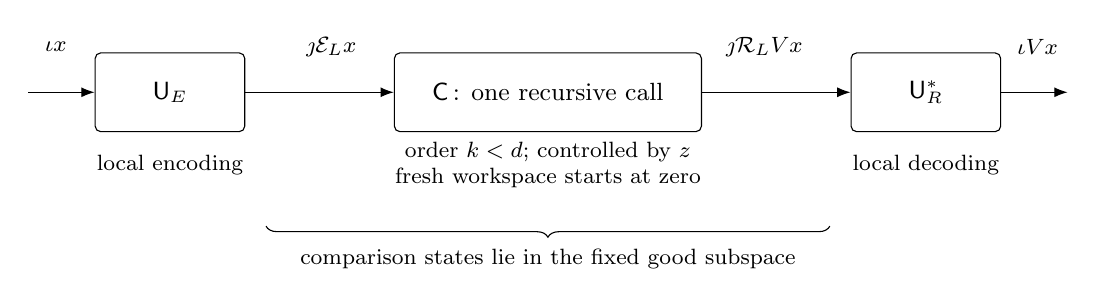
\begin{tikzpicture}[>=Latex, font=\small,
  box/.style={draw,rounded corners=2pt,minimum height=10mm,align=center},
  state/.style={align=center,font=\footnotesize}]
  \node[box,minimum width=19mm] (e) at (0,0) {$\mathsf U_E$};
  \node[box,minimum width=39mm] (f) at (4.8,0)
       {$\mathsf C$\,: one recursive call};
  \node[box,minimum width=19mm] (r) at (9.6,0) {$\mathsf U_R^*$};
  \draw[->] (-1.8,0) -- (e.west);
  \draw[->] (e.east) -- (f.west);
  \draw[->] (f.east) -- (r.west);
  \draw[->] (r.east) -- (11.4,0);
  \node[state] at (-1.45,.58) {$\iota x$};
  \node[state] at (2.05,.58) {$\jmath\mathcal E_Lx$};
  \node[state] at (7.55,.58) {$\jmath\mathcal R_LVx$};
  \node[state] at (11.02,.58) {$\iota Vx$};
  \node[state] at (0,-.92) {local encoding};
  \node[state] at (4.8,-.92) {order $k<d$; controlled by $z$\\
                           fresh workspace starts at zero};
  \node[state] at (9.6,-.92) {local decoding};
  \draw[decorate,decoration={brace,mirror,amplitude=4pt}]
       (1.22,-1.7) -- (8.38,-1.7);
  \node[state] at (4.8,-2.12)
       {comparison states lie in the fixed good subspace};
\end{tikzpicture}
\caption{One recursion level.  Labels above the arrows are the comparison
states used in Lemma~\ref{rec:step}; the intermediate states are approximate,
as quantified there.  The phase register supplies the control $z$ to the
single smaller synthesis circuit.  The local encoders contain their own
amplification rounds, while the smaller circuit occurs only once.  The map
$\iota$ initializes all work registers to zero, so the final comparison
also records their cleanup.}
\label{fig:recursion}
\end{figure}


We can now choose one set of parameters for all recursion levels.  Keep
$M,r,J$ from~\eqref{contract:parameters} and~\eqref{contract:J}, and set
\begin{equation}\label{rec:parameters}
 L=10000J,\qquad
 b=nL+\lceil\log_2(L+1)\rceil,\qquad
 K=b(L+1).
\end{equation}
Thus $K$ is the number of qubits in each field's phase register.

\begin{proposition}[Uniform programmable synthesis]\label{rec:skeleton}
Let $n\geq1$, $1\leq d\leq2^n$, and $t\geq0$.  There is a programmable-slot
circuit structure, determined by $n,d,t$, with the following property.
For every family $(U_\lambda)_{\lambda\in\{0,1\}^t}$ of unitaries on
$\C^d$, its slot tables can be chosen so that the circuit implements the
controlled unitary $U_\lambda$, preserves the labels, and has clean-workspace
operator norm error less than $1/100$ in the sense of~\eqref{slot:clean-error}.
The circuit uses
\begin{equation}\label{rec:resources}
 t+O((n+1)^{10})\quad\text{qubits},
 \qquad O((n+1)^{13})\quad\text{slots}.
\end{equation}
Its structure, including each slot's ordered control list, is generated
deterministically in time polynomial in $n+t$ from $n,d,t$.
\end{proposition}

\begin{proof}
We recurse on the valid order $d$, retaining $n$-bit index and port registers
at every level.  If $d=1$, each $U_\lambda$ is a scalar phase, implemented
exactly by one slot on an index bit that is zero throughout the valid input
subspace.

For $d\geq2$, Proposition~\ref{contract:block} gives
$V_\lambda=P_{\mathrm L,\lambda}U_\lambda P_{\mathrm R,\lambda}$ with
internal order $s$ and port order $k=d-s$.  Apply the one-step construction
of Lemma~\ref{rec:step}, prescribing the recursive family to be
$F_\lambda(z)$ and adding $z$ to the existing control labels.  Supply fresh
working qubits for this recursive circuit.  To implement $U_\lambda$, apply
$P_{\mathrm R,\lambda}^*$ before this construction and
$P_{\mathrm L,\lambda}^*$ afterward.  These transformations have exact slot
implementations, so they introduce no further error.  Their order is correct
because $P_{\mathrm L,\lambda}^*V_\lambda P_{\mathrm R,\lambda}^*=U_\lambda$.

At each step, Lemma~\ref{rec:step} adds at most
\[
 \frac{2r^L}{1-r}+10r^{2L}
 =8r^L+10r^{2L}\leq18r^L
\]
to the error of the smaller circuit.  There are fewer than $J$ steps by
Lemma~\ref{contract:depth}.  Bernoulli's inequality gives
$(4/3)^L\geq1+L/3$, and hence $r^L\leq3/L$.  The total error is therefore
\begin{equation}\label{rec:total-error}
 18Jr^L\leq\frac{54J}{L}=\frac{54}{10000}<\frac1{100}.
\end{equation}
In particular, all working qubits, including those introduced at inner
recursion levels, return to zero in the ideal comparison map.

We next count the circuit resources.  Write $N=n+1$ and
$h=\lceil\log_2(L+1)\rceil$.  Our parameters satisfy
\[
 J,L=O(N^3),\qquad b=O(N^4),\qquad K=O(N^7),\qquad h=O(N).
\]
Proposition~\ref{encode:implementation} uses $O(K+n+h)$ fresh qubits for a
pair of encoders and $O(L(K+n+h)+K)$ slots for each encoder.  The two encoders
at one level share the same register layout.  The pre- and post-conditioning
operations require only $O(n)$ more clean working qubits and slots.
All registers from an outer level remain allocated during an inner call,
so summing over the at most $J$ levels gives
\[
 t+O(J(K+n+h))=t+O(N^{10})
\]
total qubits.  Summing the slots gives
\[
 O\bigl(J[L(K+n+h)+K+n]\bigr)=O(N^{13}).
\]
These sums suffice because there is only one recursive call at a level.
The local amplification repetitions have already been included in the
factor $L$ in the encoder cost.

Finally, the structure can be generated without computing any of its table
contents.  The successive orders $d,q,s,k$ have $O(n)$-bit descriptions and
are computed in polynomial time.  Register allocations, state-preparation
bit order, Fourier transforms, reflections, and the fixed number $L$ of
amplification rounds depend only on these sizes.  Every operation depending
on $U_\lambda$---the signs, permutations, state-preparation amplitudes,
support lists, and recursively prescribed matrices---changes only a slot
table.  At most $t+O(N^{10})$ register positions occur in any ordered control
list, so writing all such lists for $O(N^{13})$ slots still takes polynomial
time in $n+t$.  No list of possible label values is generated.  This proves
both the uniformity assertion and~\eqref{rec:resources}.
\end{proof}

\section{Compilation into one Boolean oracle}\label{sec:compilation}

The skeleton of Proposition~\ref{rec:skeleton} specifies only polynomially
many slots, although each slot may have a large table. We now encode finite
gate words for those tables in one Boolean function. Two details require
care: the words must approximate matrices with their actual phases, and the
resulting circuit must be generated without finding those words. The need to
retain scalar phases under coherent control is already present in the general
controlled-gate decompositions of~\cite{Barenco1995}.

\subsection{Phase-sensitive one-qubit approximation}

We first prove the approximation fact needed for the compilation. The
argument combines the irrational-rotation proof of universality for this
gate set~\cite{Boykin2000} with the commutator refinement underlying the
Solovay--Kitaev theorem~\cite{DN2006}. The weaker polynomial bound below is
sufficient for our purpose.

\begin{lemma}\label{compile:words}
There is an absolute positive integer $K_{\mathrm w}$ such that every $S\in SU(2)$ and every
$0<\xi<1$ admit a word in $H,T,T^\dagger$ of length at most $K_{\mathrm w}\xi^{-3}$
whose matrix has determinant one and differs from $S$ by at most $\xi$ in
operator norm.
\end{lemma}

\begin{proof}
Write $X_p,Y_p,Z_p$ for the Pauli matrices, with $Y_p=iX_pZ_p$, and put
$\boldsymbol\sigma=(X_p,Y_p,Z_p)$. We first show that the determinant-one
words are dense in $SU(2)$. Up to their scalar factors,
\[
 T=e^{i\pi/8}e^{-i(\pi/8)Z_p},\qquad
 HTH=e^{i\pi/8}e^{-i(\pi/8)X_p}.
\]
Thus $W=(HTH)T=e^{i\pi/4}V$, where $V\in SU(2)$ has trace
\[
 \Tr V=2\cos^2(\pi/8)=1+\frac{\sqrt2}{2}.
\]
Recall that an algebraic integer is a root of a monic polynomial with
integer coefficients; equivalently, its monic minimal polynomial over
$\mathbb Q$ has integer coefficients. The displayed trace is not an algebraic
integer, because its monic irreducible polynomial is $x^2-2x+1/2$.
Consequently the eigenvalues of $V$ cannot be roots of unity: roots of unity
are algebraic integers, and sums of algebraic integers are algebraic integers.
Writing its eigenvalues as $e^{\pm i\theta}$, we have
$\theta/\pi\notin\mathbb Q$. The word $W^4=-V^4$ has determinant one,
and its powers are dense in the one-parameter circle about the rotation
axis of $V$.

For completeness, every matrix in $SU(2)$ has the form
$\cos t\,I+i\sin t\,\mathbf v\cdot\boldsymbol\sigma$, with
$\mathbf v\in\R^3$ a unit vector, except that the axis can be chosen
arbitrarily when $\sin t=0$. Multiplying the two rotations defining $V$
shows that its axis is not parallel to the $Z_p$ axis. Conjugation by $T$
rotates this axis through $\pi/4$ about $Z_p$, giving a nonparallel axis.
The closure of the determinant-one words contains both corresponding
circles: conjugation of a determinant-one word by $T$ is again such a word.
Rotating the second axis slightly about the first moves it out of the
plane they span. Conjugation by an element of the first circle therefore
gives a third circle with a linearly independent axis.
Let $\mathbf v_1,\mathbf v_2,\mathbf v_3$ be the three axes. The derivative
at zero of
\[
 (t_1,t_2,t_3)\longmapsto
 \prod_{j=1}^3\exp(i t_j\mathbf v_j\cdot\boldsymbol\sigma)
\]
sends $(t_1,t_2,t_3)$ to
$i(\sum_jt_j\mathbf v_j)\cdot\boldsymbol\sigma$, an isomorphism onto the
three-dimensional tangent space of $SU(2)$ at the identity. The inverse
function theorem shows that these products contain a neighborhood of the
identity. The closure of our words is thus an open subgroup. Every other
coset is open as well, so connectedness of $SU(2)$ forces this subgroup to
be all of $SU(2)$. Here connectedness also follows from the preceding
representation of $SU(2)$ as the unit sphere in $\R^4$.

We next obtain a uniform length bound. Density and compactness provide a
finite $\varepsilon_0$-net of determinant-one words of some fixed maximum
length $\ell_0$, where $\varepsilon_0>0$ will be chosen sufficiently small.
Suppose that words of length at most $\ell$ form an $\varepsilon$-net, and
choose such a word $W_0$ within $\varepsilon$ of a target $S$. The residual
$S W_0^\dagger$ has the form
\[
 S W_0^\dagger=\exp(i\mathbf a\cdot\boldsymbol\sigma),
 \qquad |\mathbf a|\le 2\varepsilon,
\]
for sufficiently small $\varepsilon$. The Pauli commutator identity gives
skew-Hermitian matrices
\[
 P=i\mathbf u\cdot\boldsymbol\sigma,\qquad
 Q=i\mathbf v\cdot\boldsymbol\sigma,
 \qquad [P,Q]=i\mathbf a\cdot\boldsymbol\sigma,
\]
with $\norm{P},\norm{Q}=O(\sqrt\varepsilon)$: take perpendicular vectors
with $\mathbf u\times\mathbf v=-\mathbf a/2$ and equal lengths.
For $A=e^P$ and $B=e^Q$, expansion of the four exponential series through
degree two gives
\[
 ABA^\dagger B^\dagger=I+[P,Q]+O(\varepsilon^{3/2})
                    =S W_0^\dagger+O(\varepsilon^{3/2}).
\]
All errors here are in operator norm with absolute constants; the remaining
terms of the exponential series are bounded by a constant times
$(\norm P+\norm Q)^3$.

Choose net words $\widetilde A,\widetilde B$ within $\varepsilon$ of
$A,B$. The gain in precision survives this substitution. Indeed,
\begin{align*}
 \norm{ABA^\dagger B^\dagger-
        \widetilde A B\widetilde A^\dagger B^\dagger}
 &\le 2\varepsilon\norm{B-I},\\
 \norm{\widetilde A B\widetilde A^\dagger B^\dagger-
        \widetilde A\widetilde B\widetilde A^\dagger\widetilde B^\dagger}
 &\le 2\varepsilon\norm{\widetilde A-I}.
\end{align*}
The first inequality follows by writing $B=I+(B-I)$ and cancelling the
identity terms; the second is the same calculation with the roles reversed.
Both right sides are $O(\varepsilon^{3/2})$. Therefore the word
\[
 \widetilde A\widetilde B\widetilde A^\dagger
 \widetilde B^\dagger W_0
\]
approximates $S$ to $C\varepsilon^{3/2}$ and has length at most $5\ell$.
Inverse words are available because $H^\dagger=H$ and both $T$ and
$T^\dagger$ belong to the alphabet.

Choose the fixed initial net so small that
$C\sqrt{\varepsilon_0}\le1/2$. Repeating the refinement $j$ times gives
error at most $2^{-j}\varepsilon_0$ and length at most $5^j\ell_0$.
Taking $j$ just large enough for the former quantity to be at most $\xi$
gives a length bounded by $K_{\mathrm w}\xi^{-3}$, since $\log_2 5<3$.
\end{proof}

Only the existence of the fixed integer $K_{\mathrm w}$ will be used. A generator can
hardcode this integer; it does not need the net or a procedure
that selects approximating words. Those selections will be stored in the
oracle.

\subsection{Lookup, control, and restoration of scratch space}

\begin{proposition}[Compilation of slots]\label{compile:slots}
Let a skeleton have $S$ slots on $Q$ qubits, and put $\eta=1/h$ for an integer
$h\ge2$.
There is a deterministic procedure, polynomial in $Q,S,1/\eta$, that produces
a circuit over $H,T,T^\dagger,\mathrm{CNOT}$ and one Boolean oracle, with
polynomially many qubits, gates, calls, and address bits. For every assignment
of the slot tables, some contents of that oracle make the circuit differ
from the prescribed skeleton by at most $S\eta$ on inputs with its added
scratch qubits zero, with the comparison circuit keeping those scratch
qubits zero.
\end{proposition}

\begin{proof}
First consider one table entry $W_y\in U(2)$. Choose a real number $\gamma_y$
and a matrix $S_y\in SU(2)$ such that
\[
 W_y=e^{i\gamma_y}S_y.
\]
By Lemma~\ref{compile:words}, choose words within $\eta/2$ of $S_y$ and of
\[
 P_y=\diag(e^{i\gamma_y},e^{-i\gamma_y}).
\]
Pad every word with identities to the common length
$\ell=\lceil K_{\mathrm w}(2/\eta)^3\rceil$. Apply the first word to the slot target
and the second to a fresh scratch qubit initially in $\ket0$. Their ideal
actions on this input multiply to $W_y$ on the target and return scratch
to zero. The two approximation errors add to at most $\eta$. Since
different $y$ occupy orthogonal control blocks, this is an operator-norm
bound for the entire controlled slot. In particular, the scalar factor
$e^{i\gamma_y}$ has been retained as a relative phase between control
values.

Use two bits to encode each symbol in $\{I,H,T,T^\dagger\}$. A single
Boolean function stores all symbol bits at addresses containing
\[
 (\text{slot number},\ y,\ \text{which word},\
   \text{word position},\ \text{symbol bit}).
\]
Pad the field for $y$ to $Q$ bits. This makes every address have a common
length $O(Q+\log(S+1)+\log(\ell+1))$. For each word position, copy the
slot's controls into the address by CNOTs, set the fixed address bits, and
query the two symbol bits into zero qubits. Apply the specified symbol
conditionally, then erase the symbol bits by querying again and reverse
the address preparation. The original slot controls do not change under
any of these target operations, so the erasure is exact even in a
superposition of control values.

We verify that symbol selection uses only the allowed elementary gates.
Bit flips are available as $HT^4H=X_p$. On bits $a,b,c$, the integer identity
\begin{equation}\label{compile:parity}
 4abc=a+b+c-(a\oplus b)-(a\oplus c)-(b\oplus c)
                         +(a\oplus b\oplus c)
\end{equation}
implements a doubly controlled $Z_p$ using $T,T^\dagger$: compute each
parity into clean scratch, apply its indicated phase, and uncompute it.
Conjugating the target by $H$ gives Toffoli. Thus equality tests on symbol
bits and all required reversible address operations are exact.
To apply $T$ conditionally, compute the AND of its control and target into
a clean scratch bit, apply $T$ there, and uncompute the AND; the same
construction applies to $T^\dagger$.

For a controlled $H$, define
\[
 D_0=(T^2H)T(T^2H)^\dagger.
\]
Because $(T^2H)Z_p(T^2H)^\dagger=Y_p$, we have
$D_0=e^{i\pi/8}e^{-i(\pi/8)Y_p}$ and hence
\[
 D_0Z_pD_0^\dagger=(X_p+Z_p)/\sqrt2=H.
\]
Apply $D_0^\dagger$ to the target, then a controlled $Z_p$, then $D_0$.
When the control is zero the two unconditional gates cancel; when it is
one their product is exactly $H$. A controlled $Z_p$ itself is a CNOT
conjugated on its target by $H$. This proves that every selected symbol,
including its phase, can be applied exactly.

It remains to compose the approximate slots. Let $A_j$ denote the actual
implementation of slot $j$, and let $V_j$ denote the ideal slot acting
trivially on all added scratch. The phase scratch may be reused. Although
its actual state need not be exactly zero after a slot, the identity
\[
 A_S\cdots A_1-V_S\cdots V_1
 =\sum_{j=1}^S A_S\cdots A_{j+1}(A_j-V_j)V_{j-1}\cdots V_1
\]
uses the error $A_j-V_j$ only after an ideal prefix. Such a prefix keeps
all added scratch at zero, precisely where the one-slot bound applies.
The unitary suffix preserves its norm. The total error is therefore at
most $S\eta$ on the claimed input subspace.

There are two words per slot, $O(\ell)$ symbol positions per word, and a
polynomial number of elementary operations per lookup. The addresses,
scratch, and total circuit size are thus polynomial in $Q,S,1/\eta$.
Generating the circuit requires only the skeleton, the fixed length bound,
and ordinary integer arithmetic. In particular, it never selects a word
or computes a table entry. Each target merely determines one admissible
Boolean function storing all choices. Adjoint slots can have their own
addresses and approximating words, or can reverse and invert stored
words; either convention uses the same single oracle.
\end{proof}

\begin{proof}[Proof of Theorem~\ref{thm:main}]
Apply Proposition~\ref{rec:skeleton} with $d=2^n$ and no initial labels.
Its skeleton has polynomially many qubits and slots, and approximates the
target unitary, including restoration of its working qubits, to error
less than $1/100$. If it has $S$ slots, compile it using
\[
 \eta=\frac{1}{100(S+1)}.
\]
Proposition~\ref{compile:slots} adds error less than $1/100$. The entire
circuit is therefore within $1/10$ in operator norm, on zero-workspace
inputs, of applying $U$ and returning every other qubit to zero. The same
polynomial bounds its width, number of gates and calls, oracle address
length, and the running time of its deterministic generator, after
increasing fixed coefficients if necessary.

Take the original index qubits as the designated outputs. For a pure input
state $\ket\psi$ together with a reference register, let $a$ and $b$ be the
actual and ideal final unit vectors before discarding workspace. The
operator-norm estimate gives $\norm{a-b}\le1/10$. Since the trace norm of
a rank-one matrix $uv^\dagger$ is $\norm u\norm v$,
\[
 \norm{aa^\dagger-bb^\dagger}_1
 \le\norm{(a-b)a^\dagger}_1+\norm{b(a-b)^\dagger}_1
 \le2\norm{a-b}\le\frac15.
\]
Partial trace cannot increase the trace norm of a Hermitian matrix, and
convexity gives the same bound for mixed input states. In particular the
supremum in Theorem~\ref{thm:main}, with its $n$-qubit reference, is at most
$1/5<1/2$.
\end{proof}

\begingroup
\small
\begin{thebibliography}{99}

\bibitem{Aaronson2021}
Scott Aaronson,
\emph{Open problems related to quantum query complexity},
ACM Transactions on Quantum Computing \textbf{2} (2021), no.~4,
Article~14, 1--9.
\href{https://doi.org/10.1145/3488559}{doi:10.1145/3488559}.

\bibitem{AK2007}
Scott Aaronson and Greg Kuperberg,
\emph{Quantum versus classical proofs and advice},
Theory of Computing \textbf{3} (2007), 129--157.
\href{https://doi.org/10.4086/toc.2007.v003a007}{doi:10.4086/toc.2007.v003a007}.

\bibitem{Barenco1995}
Adriano Barenco, Charles H.\ Bennett, Richard Cleve, David P.\ DiVincenzo,
Norman Margolus, Peter Shor, Tycho Sleator, John A.\ Smolin, and Harald Weinfurter,
\emph{Elementary gates for quantum computation},
Physical Review A \textbf{52} (1995), no.~5, 3457--3467.
\href{https://doi.org/10.1103/PhysRevA.52.3457}{doi:10.1103/PhysRevA.52.3457}.

\bibitem{BVMS2005}
Ville Bergholm, Juha J.\ Vartiainen, Mikko M\"ott\"onen, and Martti M.\ Salomaa,
\emph{Quantum circuits with uniformly controlled one-qubit gates},
Physical Review A \textbf{71} (2005), Article~052330.
\href{https://doi.org/10.1103/PhysRevA.71.052330}{doi:10.1103/PhysRevA.71.052330}.

\bibitem{Boykin2000}
P.~Oscar Boykin, Tal Mor, Matthew Pulver, Vwani Roychowdhury, and Farrokh Vatan,
\emph{A new universal and fault-tolerant quantum basis},
Information Processing Letters \textbf{75} (2000), no.~3, 101--107.
\href{https://doi.org/10.1016/S0020-0190(00)00084-3}{doi:10.1016/S0020-0190(00)00084-3}.

\bibitem{BHMT2002}
Gilles Brassard, Peter H\o yer, Michele Mosca, and Alain Tapp,
\emph{Quantum amplitude amplification and estimation},
in \emph{Quantum Computation and Information},
Contemporary Mathematics \textbf{305},
American Mathematical Society, 2002, 53--74.
\href{https://doi.org/10.1090/conm/305/05215}{doi:10.1090/conm/305/05215}.

\bibitem{DN2006}
Christopher M.\ Dawson and Michael A.\ Nielsen,
\emph{The Solovay--Kitaev algorithm},
Quantum Information \& Computation \textbf{6} (2006), no.~1, 81--95.
\href{https://doi.org/10.26421/QIC6.1-6}{doi:10.26421/QIC6.1-6}.

\bibitem{DLM2026}
Fangqi Dong, Alex Lombardi, and Fermi Ma,
\emph{Explicit separations for one-query unitary synthesis},
preprint, 2026.
\href{https://arxiv.org/abs/2607.26478}{arXiv:2607.26478}.

\bibitem{FKK2009}
Bernd Fritzsche, Victor Katsnelson, and Bernd Kirstein,
\emph{The Schur algorithm in terms of system realizations},
in D.~Alpay and V.~Vinnikov (eds.),
\emph{Characteristic Functions, Scattering Functions and Transfer Functions},
Operator Theory: Advances and Applications \textbf{197},
Birkh\"auser, 2009, 181--250.
\href{https://doi.org/10.1007/978-3-0346-0183-2_9}{doi:10.1007/978-3-0346-0183-2\_9}.

\bibitem{GSLW2019}
Andr\'as Gily\'en, Yuan Su, Guang Hao Low, and Nathan Wiebe,
\emph{Quantum singular value transformation and beyond:
exponential improvements for quantum matrix arithmetics},
Proceedings of the 51st Annual ACM SIGACT Symposium on Theory of Computing
(STOC 2019), ACM, 2019, 193--204.
\href{https://doi.org/10.1145/3313276.3316366}{doi:10.1145/3313276.3316366}.
Full version: \href{https://arxiv.org/abs/1806.01838}{arXiv:1806.01838}.

\bibitem{INNRY2022}
Sandy Irani, Anand Natarajan, Chinmay Nirkhe, Sujit Rao, and Henry Yuen,
\emph{Quantum search-to-decision reductions and the state synthesis problem},
37th Computational Complexity Conference (CCC 2022),
Leibniz International Proceedings in Informatics \textbf{234} (2022),
5:1--5:19.
\href{https://doi.org/10.4230/LIPIcs.CCC.2022.5}{doi:10.4230/LIPIcs.CCC.2022.5}.

\bibitem{LMW2024}
Alex Lombardi, Fermi Ma, and John Wright,
\emph{A one-query lower bound for unitary synthesis and breaking quantum cryptography},
Proceedings of the 56th Annual ACM Symposium on Theory of Computing
(STOC 2024), ACM, 2024, 979--990.
\href{https://doi.org/10.1145/3618260.3649650}{doi:10.1145/3618260.3649650}.

\bibitem{MVBS2005}
Mikko M\"ott\"onen, Juha J.\ Vartiainen, Ville Bergholm, and Martti M.\ Salomaa,
\emph{Transformation of quantum states using uniformly controlled rotations},
Quantum Information \& Computation \textbf{5} (2005), no.~6, 467--473.
\href{https://doi.org/10.26421/QIC5.6-5}{doi:10.26421/QIC5.6-5}.

\bibitem{NY2026}
Barak Nehoran and Henry Yuen,
\emph{All unitaries have constant depth quantum circuits},
preprint, 2026.
\href{https://arxiv.org/abs/2609.40351}{arXiv:2609.40351}.

\bibitem{Rosenthal2024}
Gregory Rosenthal,
\emph{Efficient quantum state synthesis with one query},
Proceedings of the 2024 Annual ACM--SIAM Symposium on Discrete Algorithms
(SODA), SIAM, 2024, 2508--2534.
\href{https://doi.org/10.1137/1.9781611977912.89}{doi:10.1137/1.9781611977912.89}.

\bibitem{Rosenthal2026}
Gregory Rosenthal,
\emph{Query and depth upper bounds for quantum unitaries via Grover search},
Quantum \textbf{10} (2026), Article~2144.
\href{https://doi.org/10.22331/q-2026-06-30-2144}{doi:10.22331/q-2026-06-30-2144}.

\bibitem{Tropp2018}
Joel A.\ Tropp,
\emph{Second-order matrix concentration inequalities},
Applied and Computational Harmonic Analysis \textbf{44} (2018), no.~3,
700--736.
\href{https://doi.org/10.1016/j.acha.2016.07.005}{doi:10.1016/j.acha.2016.07.005}.

\end{thebibliography}

\endgroup
\end{document}
